\documentclass{article}
\usepackage{amsmath}
\usepackage{geometry}
\usepackage{float}
\geometry{a4paper, left=2cm, right=2cm, top=2.54cm, bottom=2.54cm}
\usepackage{indentfirst}
\usepackage{enumitem}
\usepackage{bm}
\usepackage[hidelinks]{hyperref}

% 段落間距  (begin doc 才設定)
\usepackage{parskip}
    % 普通文字,行距
    \usepackage[onehalfspacing]{setspace}
    
\usepackage{tabularx}

\usepackage{fontspec,xltxtra,xunicode}

\usepackage{titlesec}

\def\Large{\fontsize{18}{10}\selectfont}
\def\huge{\fontsize{26}{10}\selectfont}
\def\Huge{\fontsize{36}{30}\selectfont}

\titleformat{\section}
  {\fontsize{16pt}{15}\bfseries}
  {\selectfont\thesection.}
  {0.5em}
  {}

\titleformat{\subsection}
  {\fontsize{14pt}{15}\bfseries}
  {\selectfont\thesubsection.}
  {0.5em}
  {}


\usepackage{xeCJK}
\setCJKmainfont[AutoFakeBold=3]{DFKai-SB} %设置中文字体\XeTeXlinebreaklocale “zh”\XeTeXlinebreakskip = 0pt plus 1pt minus 0.1pt %文章内中文自动换行


\usepackage{minted}
\setminted{
baselinestretch=1,
fontsize=\small,
python3=true,
style = tango,
}


\usepackage{caption}
\newenvironment{code}{\captionsetup{type=listing, font=large}}{}

\captionsetup{font=large}



\usepackage{longtable}
\usepackage{array}
\usepackage{makecell}
\renewcommand{\arraystretch}{1.2}

% % 首行縮排
% \usepackage{indentfirst}
% % 首行縮排距離
% \setlength\parindent{28pt}

\renewcommand{\figurename}{Fig.}

\setmainfont{Times New Roman}

\title{\textbf{{\huge Final Project} \\ 記憶體積體電路\ Memory\ Circuit\ Design}}
\author{{\Large\textbf{ 電機4A\quad 109501201\quad 陳緯亭}}}
\date{\Large{\today}} 



\begin{document}

% 首行縮排距離
\setlength\parindent{28pt}

% 段落後間距
\setlength\parskip{14pt}



\newcolumntype{L}[1]{>{\raggedright\let\newline\\\arraybackslash\hspace{0pt}}m{#1}}
\newcolumntype{C}[1]{>{\centering\let\newline\\\arraybackslash\hspace{0pt}}m{#1}}
\newcolumntype{R}[1]{>{\raggedleft\let\newline\\\arraybackslash\hspace{0pt}}m{#1}}


\maketitle
\vspace*{-0.5cm}

\fontsize{12pt}{1.5em}

\selectfont

\section{Construct the circuitry schematic layout of the 16-nm FinFET 6T SRAM Unit Cell.}

Layout 盡可能密集,不要太分散。

\begin{figure}[H]
\centering
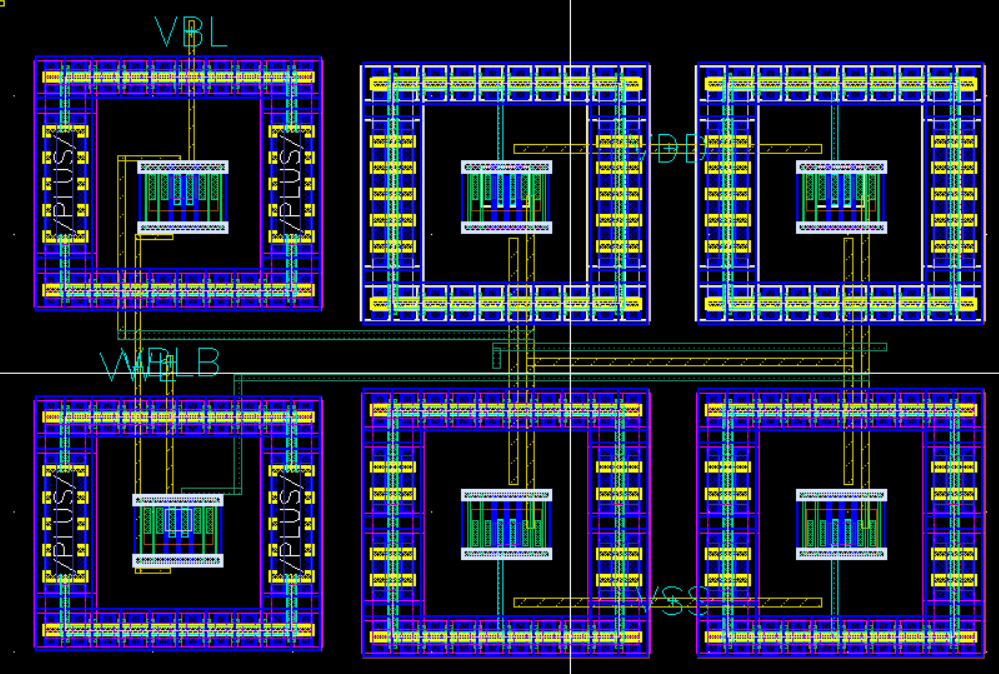
\includegraphics[width=\linewidth]{./img/2024-01-05-14-52-06.png}
\caption{Layout of the 16-nm FinFET 6T SRAM Unit Cell}
\end{figure}

\section{Provide the proof screen-copy picture of the DRC and LVS
verification for your layout.}

\begin{figure}[H]
\centering
\begin{minipage}[t]{0.45\textwidth}
\centering
    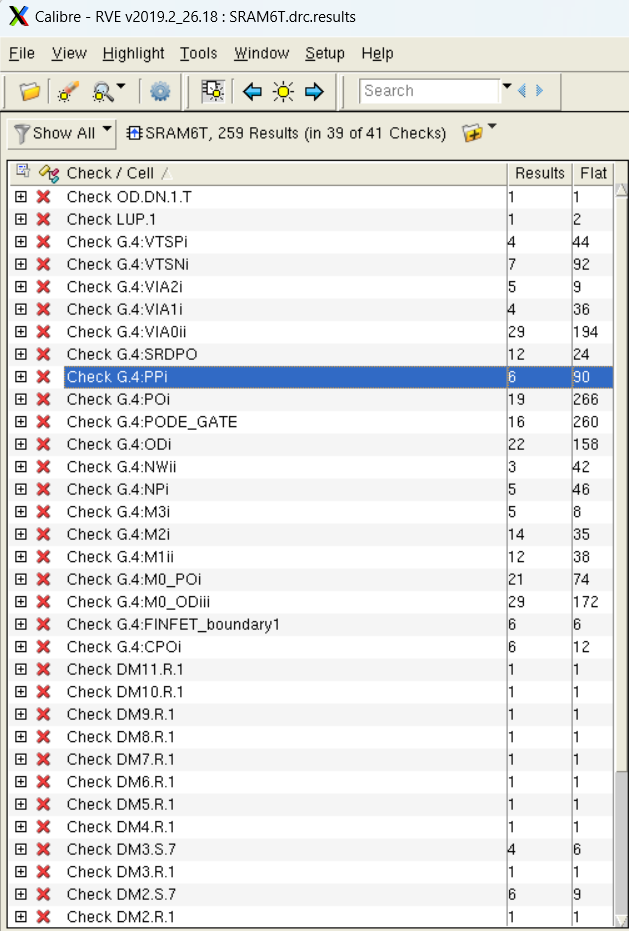
\includegraphics[width=\linewidth]{./img/2024-01-05-15-01-42.png}
\caption{DRC.results}
\label{filter}
\end{minipage}
\qquad
\begin{minipage}[t]{0.45\textwidth}
\centering
    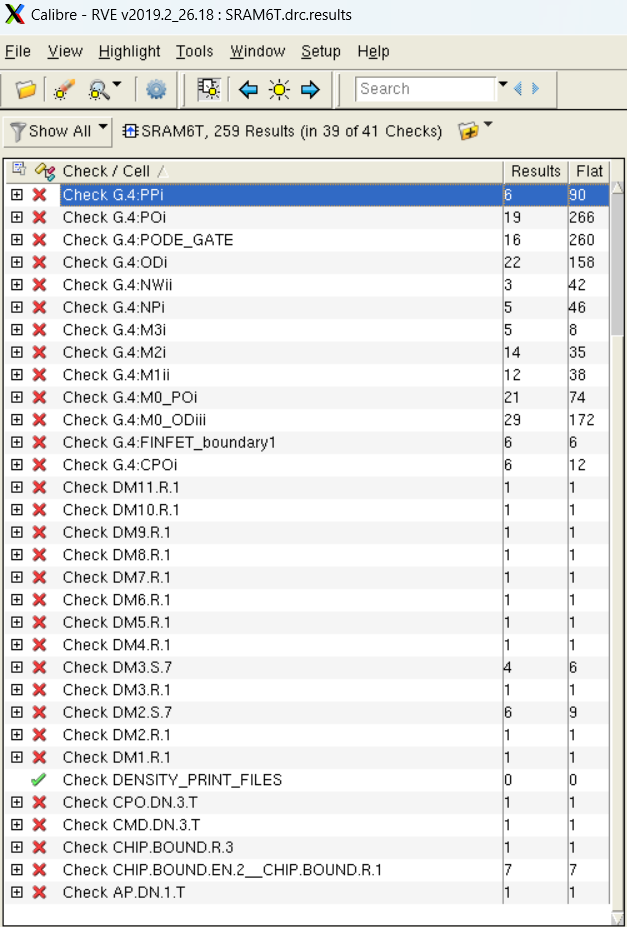
\includegraphics[width=\linewidth]{./img/2024-01-05-15-01-54.png}
\caption{DRC.results}
\label{db10}
\end{minipage}
\end{figure}

\begin{figure}[H]
  \centering
  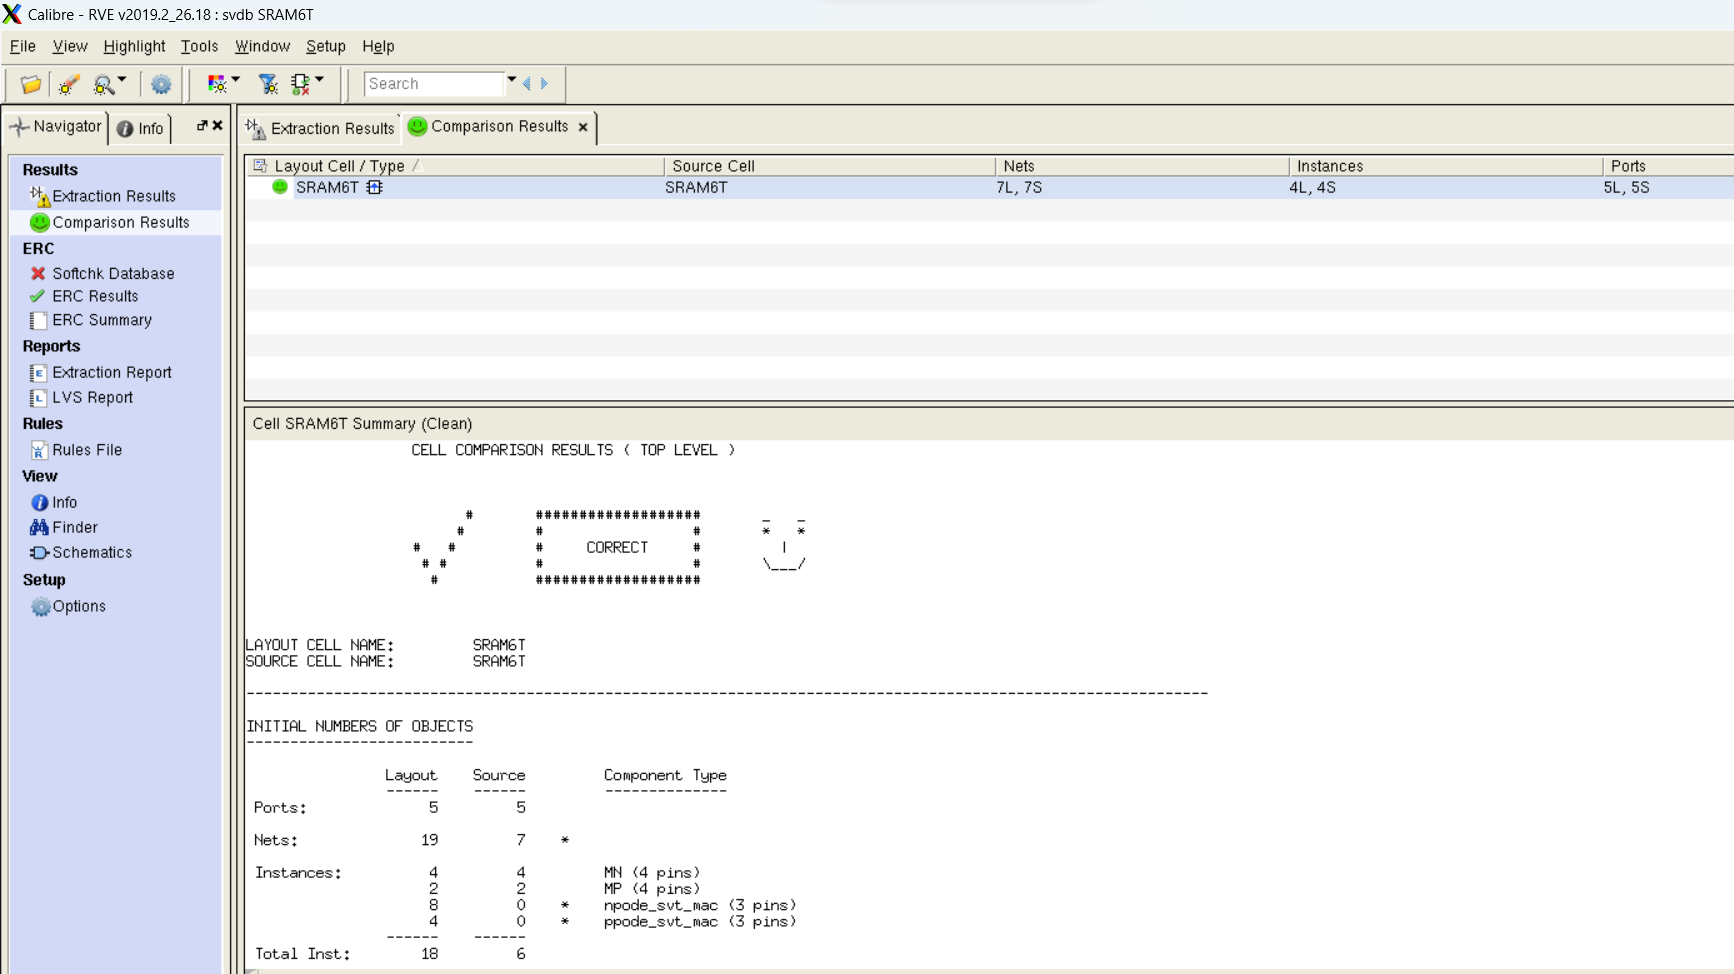
\includegraphics[width=0.9\linewidth]{./img/2024-01-05-15-00-11.png}
  \caption{LVS.results}
  \end{figure}


\section{Plot the RSNM and WNM of the 16-nm FinFET 6T SRAM unit cell with Vdd=0.8V, 0.6V, 0.4V.}

\begin{figure}[H]
  \centering
  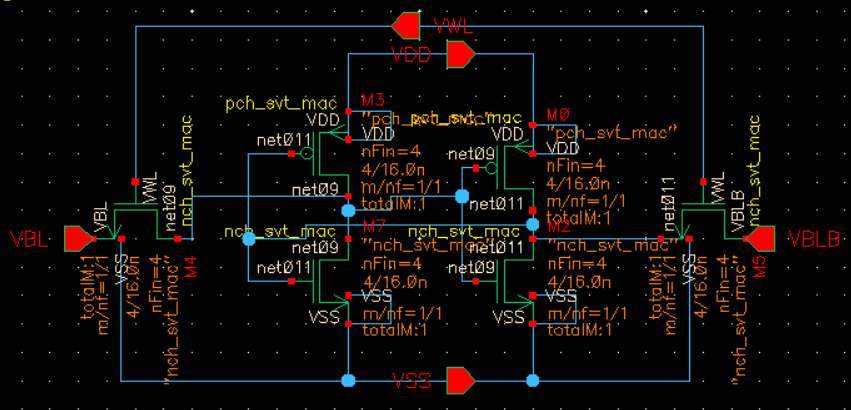
\includegraphics[width=0.9\linewidth]{./img/2024-01-11-10-29-38.png}
  \caption{16-nm FinFet 6T SRAM schematic}
  \end{figure}

\subsection{Vdd=0.8V}

對 Vdd = 0.8V , RSNM = 0.217 V , WNM = 0.480 V。

\begin{figure}[H]
  \centering
  \begin{minipage}[t]{0.45\textwidth}
  \centering
      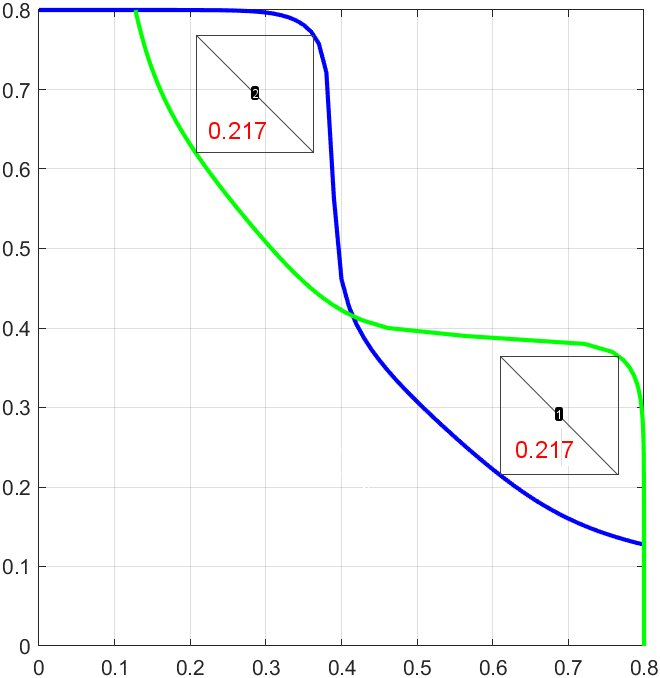
\includegraphics[width=\linewidth]{./img/2024-01-11-22-57-21.png}
  \caption{RSNM}
  \label{r8}
  \end{minipage}
  \qquad
  \begin{minipage}[t]{0.45\textwidth}
  \centering
      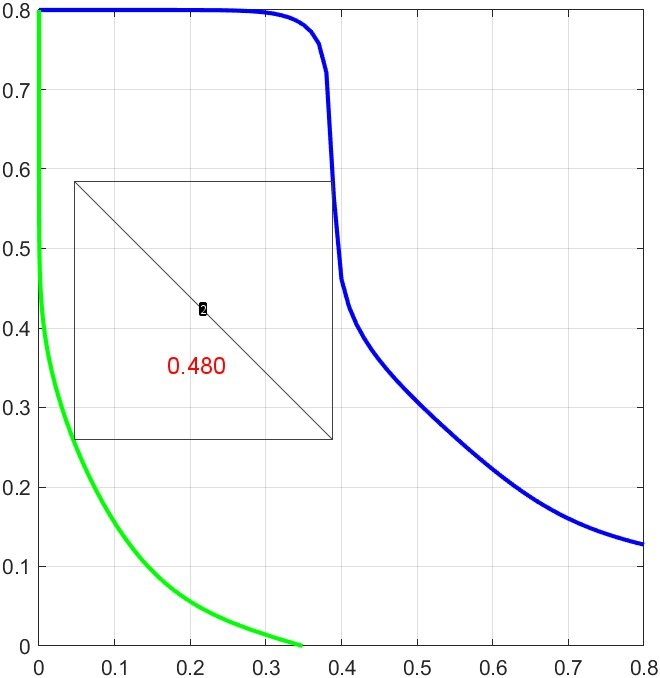
\includegraphics[width=\linewidth]{./img/2024-01-11-23-03-30.png}
  \caption{WNM}
  \label{w8}
  \end{minipage}
  \end{figure}

  \subsection{Vdd=0.6V}

  對 Vdd = 0.6V , RSNM = 0.173 V , WNM = 0.365 V。

  \begin{figure}[H]
    \centering
    \begin{minipage}[t]{0.45\textwidth}
    \centering
        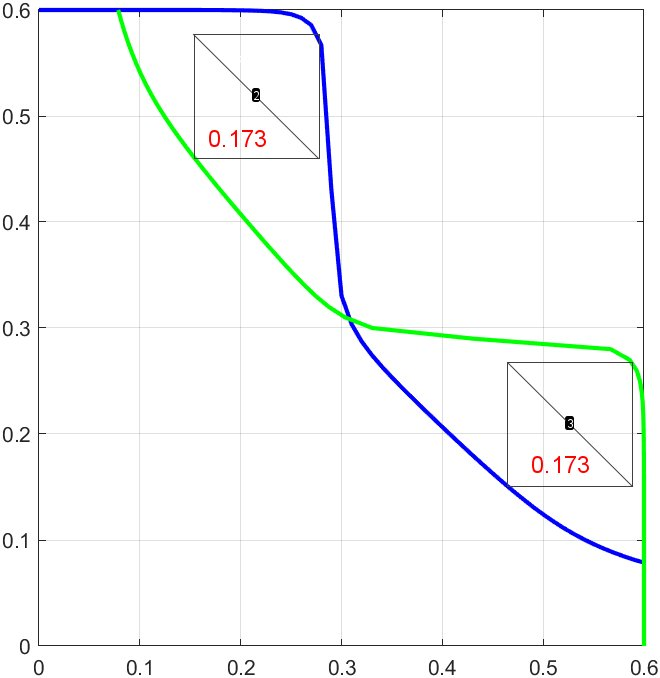
\includegraphics[width=\linewidth]{./img/2024-01-11-23-24-50.png}
    \caption{RSNM}
    \label{r6}
    \end{minipage}
    \qquad
    \begin{minipage}[t]{0.45\textwidth}
    \centering
        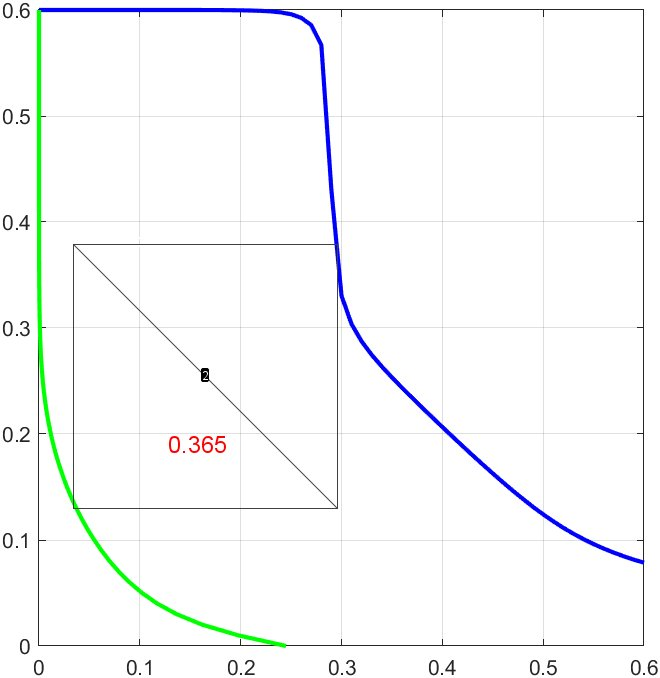
\includegraphics[width=\linewidth]{./img/2024-01-11-23-25-06.png}
    \caption{WNM}
    \label{w6}
    \end{minipage}
    \end{figure}

    \subsection{Vdd=0.4V}

    對 Vdd = 0.4V , RSNM = 0.108 V , WNM = 0.263 V。

    \begin{figure}[H]
      \centering
      \begin{minipage}[t]{0.45\textwidth}
      \centering
          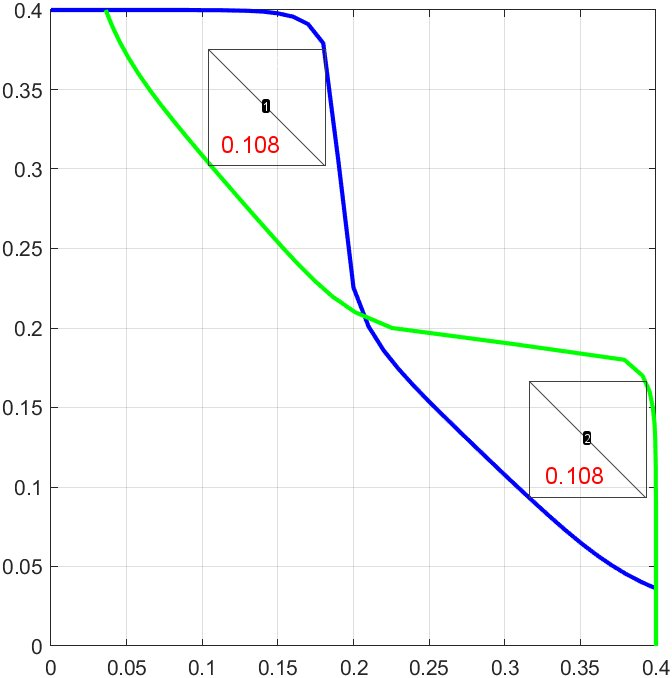
\includegraphics[width=\linewidth]{./img/2024-01-11-23-35-36.png}
      \caption{RSNM}
      \label{r4}
      \end{minipage}
      \qquad
      \begin{minipage}[t]{0.45\textwidth}
      \centering
          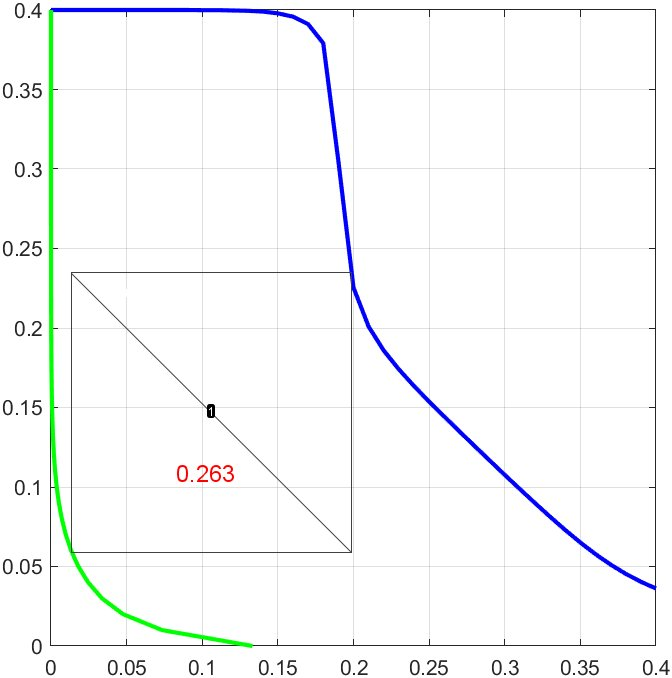
\includegraphics[width=\linewidth]{./img/2024-01-11-23-32-16.png}
      \caption{WNM}
      \label{w4}
      \end{minipage}
      \end{figure}

      根據Fig.~\ref{r8}、Fig.~\ref{r6}、Fig.~\ref{r4}可以發現RSNM 會隨著,VDD 變小逐漸
      變小,與之成正比。而且因為Voltage dividend 的關係,在圖形開頭與結尾處
      會有一個空白區間。根據 Fig.~\ref{w8}、Fig.~\ref{w6}、Fig.~\ref{w4} 可以發現WNM 也會隨著,VDD 變小逐漸變小,與之成正比。通常在同一VDD 下,RSNM 都會小於
      WNM。


\end{document}